% !TEX root = ../DP_Vik_Tomas_2013.tex
\chapter{Implementace}
Pro lepší představu bude nejdříve zběžně popsán způsob, jakým se všeobecně sestavuje aplikace ve frameworku Ruby on Rails. Následně se bude kapitola věnovat detailněji implementaci napojení aplikace na srovnávač Heureka.cz, implementací získávání aktuálních cen a jejich zpracování do grafu a kapitolu uzavře ukázka implementovaných obrazovek aplikace.

\section{Standardní rozvržení aplikace v Ruby on Rails}
Jak již bylo řečeno v kapitole \ref{sec:ror}, aplikace upřednostňuje konvenci před konfiguraci, což na jednu stranu znamená minimum konfigurace aplikace, na druhou stranu to znamená, že má vývojář přesně dané postupy jak v implementaci něčeho dosáhnout. Framework je postaven na návrhovém vzoru MVC a díky tomu je aplikace rozdělena na tři významné části.

\subsection{Model}
Model reprezentuje informace v aplikaci a pravidla jak s nimi zacházet. Což se dá interpretovat také jako mechanismus zapisování a čtení databáze a pravidla tohoto zápisu/čtení. Model je v Rails řešen pomocí knihovny Active Record. Ta poskytuje nad každým objektem modelu velkou škálu funkcí které manipulují přímo s databází. Každá modelová třída musí dědit od |ActiveRecord::Base|. Na schématu \ref{fig:model-diagram} jsou vidět všechny modelové třídy ve výsledné aplikaci. Každý model v Rails má v příslušné tabulce v databázi ještě dva sloupce |create_at| a |updated_at| jejichž hodnoty se automaticky nastavují při vytvoření/upravení záznamu.

\begin{figure}[htb]
\begin{center}
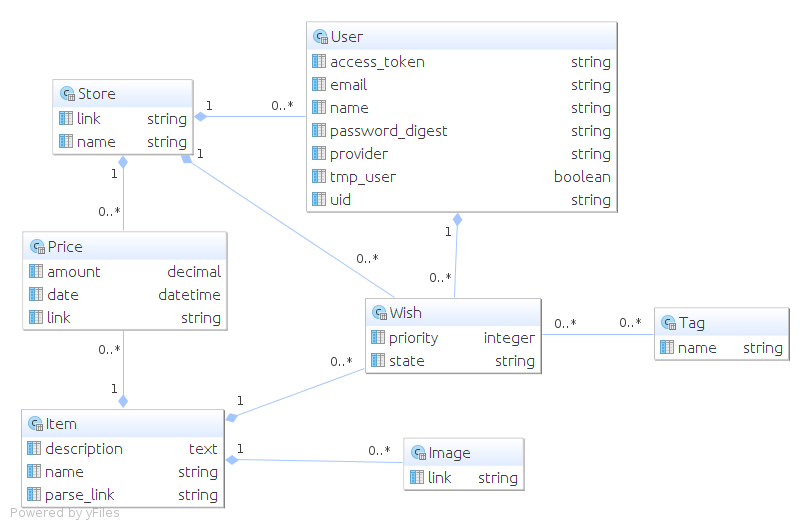
\includegraphics[width=120mm]{./pictures/model-diagram.png}
\caption{Diagram tříd v modelu aplikace}
\label{fig:model-diagram}
\end{center}
\end{figure}

\subsection{Controller}
Controller je v Rails třída, která dědí od třídy |ActionController::Base|. Tato třída má na starosti zpracování HTTP dotazů. Pokud přijde dotaz, framework se pokusí v routes souboru\footnote{Konfigurační soubor, ve kterém jsou nastaveny pro každou validní URL odpovídající controllery a jejich metody.} najít vhodný controller a jeho metodu, kterou poté zavolá. Controller má mimo jiné přístup k parametrům, se kterými byl proveden HTTP dotaz a k session proměnné.

Dále je v Rails aplikacích standardem, že existuje controller, který se nazývá |ApplicationController| a od něj dědí všechny ostatní controllery. Tak je tomu i ve výsledné aplikaci.

V následující ukázce je kus kódu největšího controlleru výsledné aplikace |WishesController|. Konkrétně metoda, která se volá po odeslání formuláře na přidání přání.

\lstset{language = ruby, style=custom}
\begin{lstlisting}
class WishesController < ApplicationController

#....... kod vynechan

  # POST /wishes
  # POST /wishes.json
  def create
    #ziskame prani pro id z parametru
    @wish = Wish.new(params[:wish])
    #z retezce ziskame stitky
    tags = Tag.parse_tags(params[:tags])
    @wish.tags = tags
    @wish.user = current_user
    #inicializujeme prioritu prani
    @wish.initialize_priority(params[:user_priority].to_d)
    respond_to do |format|
      format.html { redirect_to wishes_path, notice: :success }
      format.json { render json: @wish, status: :created, location: @wish }
    end
  end

#....... kod vynechan

end
\end{lstlisting}

\subsection{View}
View reprezentuje uživatelské rozhraní aplikace a v Rails je řešeno pomocí HTML souborů, do kterých jsou vloženy části Ruby kódu. View  je tedy ta část aplikace, která poskytuje data klientskému prohlížeči.

View je vykreslován controllerem a má také k dispozici všechna data, která má k dispozici controller. Proto je snadné předávat do view data získaná v controlleru.

Následuje ukázka kódu view, který má ve výsledné aplikaci na starost vykreslení seznamu štítků v levém panelu.

\lstset{language = html, style=custom}
\begin{lstlisting}
<div id="tag-overview" class="sidebar-nav">
  <div class="well">
    <ul class="nav nav-stacked nav-pills">
      <li class="nav-header">Stitky</li>
      <!-- Iterace pres kazdy stitek s jeho indexem -->
      <% @main_page_tags.each_with_index do |tag, index| %>
        <!-- pokud je to paty a vicery stitek, nebue na zacatku zobrazen -->
        <li <%= 'class=overflow' if index > 4  %>>
          <a href="/wishes/bytag/<%= tag.name %>">
            <%= truncate(tag.name, length: 12) %> <%= raw(ApplicationHelper.badge(tag.wish_count(current_user.id))) %>
          </a>
        </li>
      <% end %>
      <!-- Tlacitko pro zobrazeni zbyvajicich stitku -->
      <% if @main_page_tags.size > 4 %>
          <li><a id="more-tags-button" class="more" href="#"><i class="icon-chevron-down"></i>Vice</a></li>
      <% end %>
    </ul>
  </div>
</div>
\end{lstlisting}

\section{Napojení výsledné aplikace na srovnávač Herueka.cz}
Jako zdroj dat pro aplikaci je využit server pro srovnávání cen \textbf{Heureka.cz} a způsob získávání dat z tohoto serveru je \textbf{Web scraping}. Pro usnadnění získávání dat z webových stránek je použita knihovna Nokogiri\footnote{\url{http://nokogiri.org/}}.

Získávání dat spočívá v dotazování na specifické URL serveru. To má vždy stejnou podobu, například získání dokumentu s výsledky hledání produktu vypadá následovně:

\lstset{language = ruby, style=custom}
\begin{lstlisting}
doc = Nokogiri::HTML(open("http://www.heureka.cz/?h[fraze]=#{heureka_term}"))
\end{lstlisting}

\noindent kde |heureka_term| je vyhledávaný výraz.

V takto získaném dokumentu je snadné hledat jednotlivé elementy pomocí CSS selektorů (viz. \ref{sec:css-selektor}) a číst obsah takto získaných elementů pomocí metody. Následuje ukázka kódu\footnote{Pro přehlednost bylo z ukázky odebráno přiřazení získaných dat.} na získání produktů z vyhledávání provedeného předchozím příkazem:

\begin{lstlisting}
products = doc.css('#content #search .product')
products.each do |product|
  image_link = product.css('.foto img').first['src']
  description_document = product.css('.desc p.small').first
  if description_document
    search_item.description = description_document.content
  end
  item_link = product.css('div h2 a').first
  #nazev produktu
  name = item_link.content
  #odkaz na tento produkt, ze ktereho se prani ziska
  parse_link = item_link['href']
  #pokud odkaz nevede na heureku => neslo by parsovat dalsi data
  next if search_item.parse_link.include? 'exit'
  price_from_to = product.css('.wherebuy .price a.pricen').first.content
  price_from = price_from_to.split('-').first.gsub(/[^0-9]/i, '')
  price_to = price_from_to.split('-').last.gsub(/[^0-9]/i, '')
end
\end{lstlisting}

Základními metodami naimplementované knihovny pro získávání dat ze serveru Heureka.cz jsou:

\begin{itemize}
\item |search_term(term, limit)| - vrátí vyhledané produkty, tyto produkty nejsou ještě vloženy do databáze, každý vyhledaný produkt obsahuje URL, ze kterého je možné jeho data získat
\item |parse_item(item_url)| - je volána při přidávání přání s novým produktem, získá z dané URL produkt, uloží všechny jeho informace do databáze a vrátí jej
\item |get_prices(item)| - volá se při vytváření nového přání a poté periodicky každý den. Získá ceny ze všech obchodů, ve kterých se produkt z~parametru prodává.
\end{itemize}

Při implementaci získávání dat metodou Web Scraping bylo nejobtížnější ošetřit všechny možné podoby stránek, které server vrací. Např. videa v galerii obrázků, chybějící popis nebo obrázek produktu apod.

\section{Získávání cen a sestavování grafu vývoje ceny}
Způsob získávání cen je ve výsledné aplikaci osvozen od způsobu, jakým se získávají data ze stránek srovnávače Heureka.cz. Ceny jsou načítány ze zdroje dat jednou denně. V datovém modelu (viz. \ref{fig:model-diagram}) je u každého produktu pole s URL adresou. Na ní je stránka srovnávače Heureka.cz, kde jsou informace o cenách produktu v jednotlivých obchodech. Aplikace projde všechny produkty a z této stránky k nim načte příslušné informace.

Graf vývoje ceny je sestavován na základě periodických dat o ceně uložených v databázi. Pole s daty grafu se vytváří následujícím způsobem: 
\begin{lstlisting}
#pole poslednich 7mi dni
days = (6.days.ago.to_date..Date.today).to_a
hash = Hash.new
#prochazime pole postupne (zaciname dneskem) a pro kazdy den ziskame nejnizsi cenu a cenu ve vybranem obchode
days.reverse_each do |day|
  low_price = Price.where(:item_id => item.id, :created_at => day.at_beginning_of_day..day.tomorrow.at_beginning_of_day).order('amount ASC').first
  store_price = Price.where(:item_id => item.id, :store_id => selected_store.id, :created_at => day.at_beginning_of_day..day.tomorrow.at_beginning_of_day).order('amount ASC').first
  #ukoncime, pokud databaze cenu neobsahuje (prani neni v databazi dostatecny pocet dni)
  break if !low_price
  hash[day] = [low_price.amount.to_i, store_price.amount.to_i]
end
\end{lstlisting}

Výsledkem tohoto kódu je mapa, ve které je klíčem den a hodnotou je pole s nejnižší a vybranou cenou. Jinými slovy mapa obsahuje pro každý den dvojici cen, celkově nejnižší a cenu z vybraného obchodu. Tento objekt je po dalších drobných úpravách předán Google Visualization API\footnote{\url{https://developers.google.com/chart/interactive/docs/gallery/linechart}}, které z něj vytvoří SVG dynamický graf umístěný na výsledné stránce.

V implementaci je vidět zásadní problém, který skrývá metoda Web Scraping. Data o cenách se k produktům donačítají postupně každý den. To znamená, že pokud uživatel přidá do aplikace produkt, který před ním nikdo nepřidal, je u tohoto produktu uložena cena pouze za poslední den. Plný graf vývoje ceny přání uživatel uvidí až po týdnu.

\section{Výsledné grafické uživatelské rozhraní.}
Grafické rozhranní aplikace je hodně ovlivněné základním vzhledem Twitter Bootstrap frameworku. Pro ukázku implementace byly vybrány 2 relativně nejsložitější obrazovky aplikace.
\subsection{\ref{sc-11}}
Při implementaci bylo rozložení prvků striktně dodržen wireframe návrh (kapitola \ref{sec:wireframe-pridani-prani}). Ovládací prvky obrazovky jsou co nejintiutivněji barevně rozlišeny. Např. vysoká priorita má červenou barvu a nízká zelenou. Obrázky lze přepínat kliknutím na miniaturu. Obchod lze vybrat tlačítkem \emph{Zvolte obchod}.

Výsledná implementace je vidět na obrázku \ref{fig:impl-add}.
\begin{figure}[htb]
\begin{center}
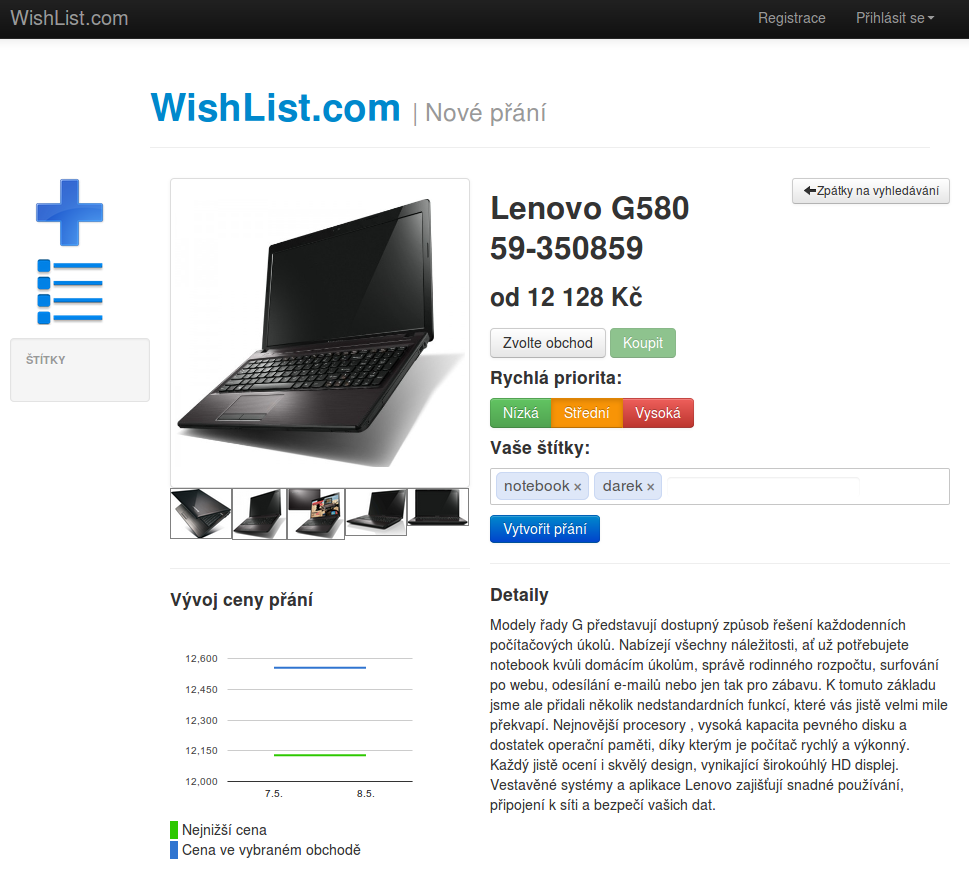
\includegraphics[width=100mm]{./pictures/impl-add.png}
\caption{Implementace obrazovky: \ref{sc-11}}
\label{fig:impl-add}
\end{center}
\end{figure}

Na implementované obrazovce je také vidět horní lišta, která indikuje, že uživatel není přihlášený a umožňuje mu se buďto přihlásit, nebo zaregistrovat. Všechny ostatní ovládací prvky umožňující provést hlavní akce aplikace (kapitola \ref{sec:hlavni-akce}) jsou zde také přítomny.

\subsection{\ref{sc-04}}
Návrh, podle kterého implementace probíhala je vidět v kapitole \ref{sec:wireframe-vsechna-prani}. Uživatel má na jedné obrazovce zobrazena všechna svá přání seřazená podle priority od nejvyšší po nejnižší. Měnit prioritu přání je možné jednoduchým přetažením přání na jiné místo.

V implementaci je zároveň vidět levý panel se štítky jehož návrh je popsán v kapitole \ref{sec:hlavni-ovladaci-prvky}. Z tohoto panelu lze snadno přejít na zobrazení všech přání obsahujících daný štítek.

\begin{figure}[htb]
\begin{center}
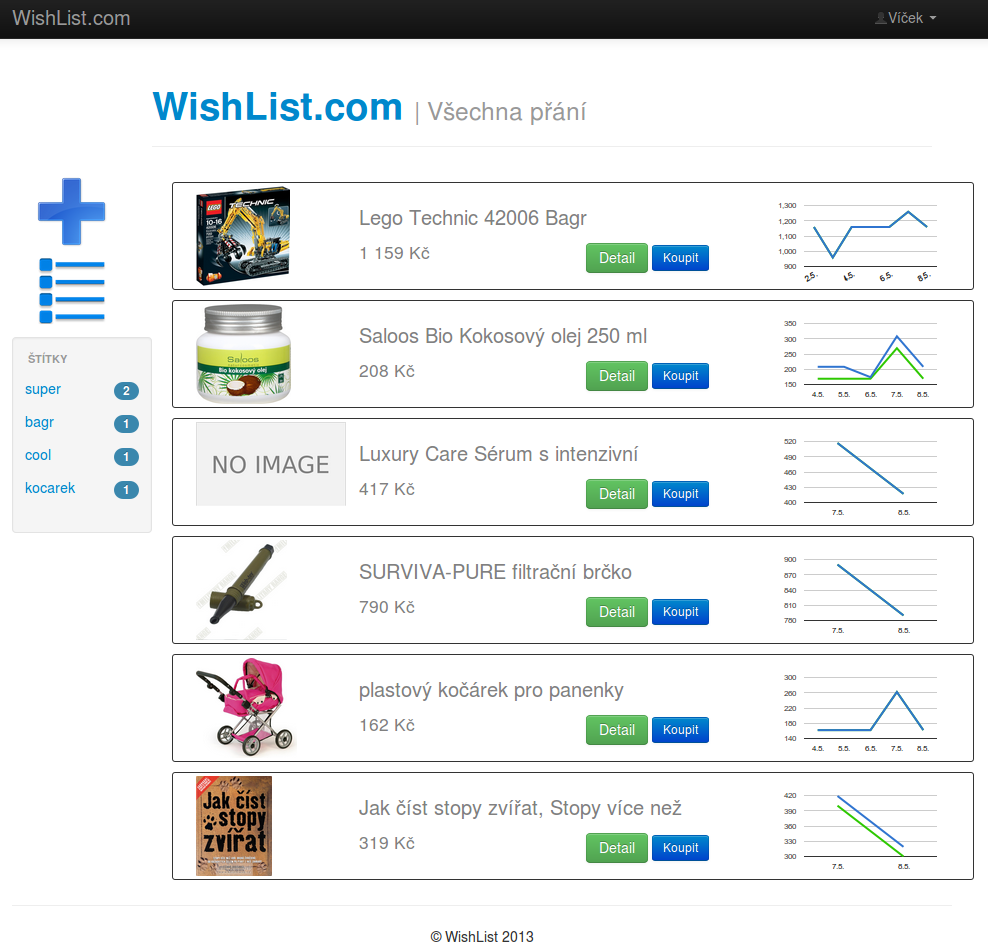
\includegraphics[width=100mm]{./pictures/impl-all.png}
\caption{Implementace obrazovky: \ref{sc-04}}
\label{fig:impl-all}
\end{center}
\end{figure}